\documentclass{article}[18pt]
\ProvidesPackage{format}
%Page setup
\usepackage[utf8]{inputenc}
\usepackage[margin=0.7in]{geometry}
\usepackage{parselines} 
\usepackage[english]{babel}
\usepackage{fancyhdr}
\usepackage{titlesec}
\hyphenpenalty=10000

\pagestyle{fancy}
\fancyhf{}
\rhead{Sam Robbins}
\rfoot{Page \thepage}

%Characters
\usepackage{amsmath}
\usepackage{amssymb}
\usepackage{gensymb}
\newcommand{\R}{\mathbb{R}}

%Diagrams
\usepackage{pgfplots}
\usepackage{graphicx}
\usepackage{tabularx}
\usepackage{relsize}
\pgfplotsset{width=10cm,compat=1.9}
\usepackage{float}

%Length Setting
\titlespacing\section{0pt}{14pt plus 4pt minus 2pt}{0pt plus 2pt minus 2pt}
\newlength\tindent
\setlength{\tindent}{\parindent}
\setlength{\parindent}{0pt}
\renewcommand{\indent}{\hspace*{\tindent}}

%Programming Font
\usepackage{courier}
\usepackage{listings}
\usepackage{pxfonts}

%Lists
\usepackage{enumerate}
\usepackage{enumitem}

% Networks Macro
\usepackage{tikz}


% Commands for files converted using pandoc
\providecommand{\tightlist}{%
	\setlength{\itemsep}{0pt}\setlength{\parskip}{0pt}}
\usepackage{hyperref}

% Get nice commands for floor and ceil
\usepackage{mathtools}
\DeclarePairedDelimiter{\ceil}{\lceil}{\rceil}
\DeclarePairedDelimiter{\floor}{\lfloor}{\rfloor}

% Allow itemize to go up to 20 levels deep (just change the number if you need more you madman)
\usepackage{enumitem}
\setlistdepth{20}
\renewlist{itemize}{itemize}{20}

% initially, use dots for all levels
\setlist[itemize]{label=$\cdot$}

% customize the first 3 levels
\setlist[itemize,1]{label=\textbullet}
\setlist[itemize,2]{label=--}
\setlist[itemize,3]{label=*}

% Definition and Important Stuff
% Important stuff
\usepackage[framemethod=TikZ]{mdframed}

\newcounter{theo}[section]\setcounter{theo}{0}
\renewcommand{\thetheo}{\arabic{section}.\arabic{theo}}
\newenvironment{important}[1][]{%
	\refstepcounter{theo}%
	\ifstrempty{#1}%
	{\mdfsetup{%
			frametitle={%
				\tikz[baseline=(current bounding box.east),outer sep=0pt]
				\node[anchor=east,rectangle,fill=red!50]
				{\strut Important};}}
	}%
	{\mdfsetup{%
			frametitle={%
				\tikz[baseline=(current bounding box.east),outer sep=0pt]
				\node[anchor=east,rectangle,fill=red!50]
				{\strut Important:~#1};}}%
	}%
	\mdfsetup{innertopmargin=10pt,linecolor=red!50,%
		linewidth=2pt,topline=true,%
		frametitleaboveskip=\dimexpr-\ht\strutbox\relax
	}
	\begin{mdframed}[]\relax%
		\centering
		}{\end{mdframed}}



\newcounter{lem}[section]\setcounter{lem}{0}
\renewcommand{\thelem}{\arabic{section}.\arabic{lem}}
\newenvironment{defin}[1][]{%
	\refstepcounter{lem}%
	\ifstrempty{#1}%
	{\mdfsetup{%
			frametitle={%
				\tikz[baseline=(current bounding box.east),outer sep=0pt]
				\node[anchor=east,rectangle,fill=blue!20]
				{\strut Definition};}}
	}%
	{\mdfsetup{%
			frametitle={%
				\tikz[baseline=(current bounding box.east),outer sep=0pt]
				\node[anchor=east,rectangle,fill=blue!20]
				{\strut Definition:~#1};}}%
	}%
	\mdfsetup{innertopmargin=10pt,linecolor=blue!20,%
		linewidth=2pt,topline=true,%
		frametitleaboveskip=\dimexpr-\ht\strutbox\relax
	}
	\begin{mdframed}[]\relax%
		\centering
		}{\end{mdframed}}
\lhead{Software Engineering}


\begin{document}
\begin{center}
\underline{\huge SD Methodologies III}
\end{center}
\section{SCRUM}
\subsection{Sprint}
\begin{center}
	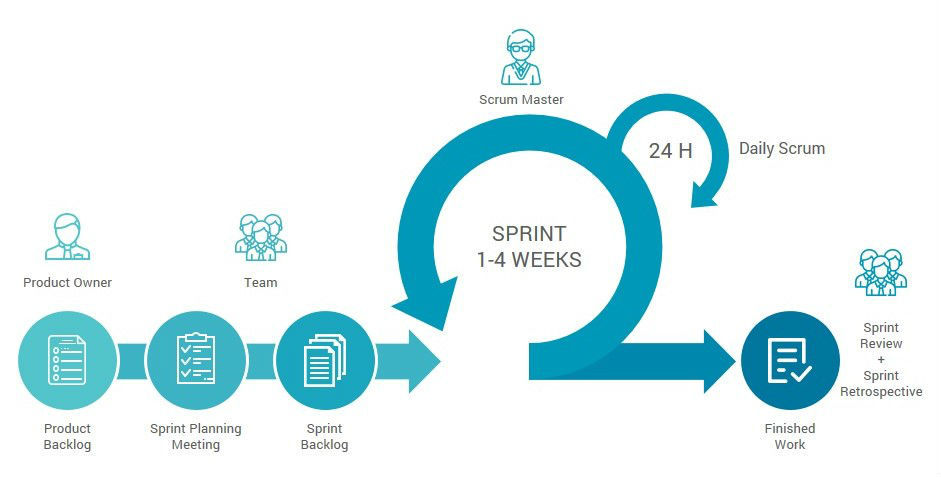
\includegraphics[scale=0.7]{sprint}
\end{center}
\begin{itemize}
	\item The starting point for planning is the product backlog (user stories), which is the list of work to be done on the project
	\item Once these are agreed, the team organise themselves to develop the software - the team creates a spring backlog (their to-do list for the sprint). At the end of the sprint, the work done is reviewed and presented to stakeholder. The next sprint cycle then begins
\end{itemize}
\subsection{Artifacts}
\begin{defin}[Scrum Product Backlog (SPB)]
	A list of all things that need to be done within the project. It replaces the traditional requirements specification artifacts. These items can have a technical nature or can be user-centric e.g. in the form of user stories
\end{defin}
\begin{itemize}
	\item Each scrum product backlog has certain properties that differentiate it from a simple to-do list:
	\begin{itemize}
		\item An entry in the SPB always add value for the customer
		\item The entries in the SPB are prioritized and ordered accordingly
		\item All entries are estimated
		\item The SPB is a living document (priorities shift)
		\item There are no action-items or low-level tasks in the SPB
		\item SPB entries can be scenarios or use cases
	\end{itemize}
\end{itemize}
\subsection{SPB items (SPBI)}
\begin{itemize}
	\item What you have agreed to do (SPBI) in the current sprint; has an end
	\item How is breaking the SPBIs into small pieces - sprint tasks
	\item These tasks can be tested
\end{itemize}
\subsection{Meetings}
Sprint planning:
\begin{itemize}
	\item Plan one sprint. PO and team decide what SPBIs go into sprint backlog (have top priorities); try to get it clear what they have to do and how much they can do in the time allocated (timebox)
	\item Use story points - arbitrary measure of effort required
\end{itemize}
Daily scrum:
\begin{itemize}
	\item Meet daily; 15 minute stand up and report to each other NOT to the PO or SM
	\item What you did yesterday, what you will do today, what problems have you got
\end{itemize}
Sprint review:
\begin{itemize}
	\item Demo potentially shippable product increment to PO and anyone interested. PO declares what is complete and what doesn't satisfy user requirements
\end{itemize}
Retrospective meeting:
\begin{itemize}
	\item At the end of every sprint what went well, what can be improved, what you have learned, feedback to each other - teams take ownership of the process
\end{itemize}
Refinement meeting:
\begin{itemize}
	\item Team and PO look ahead a little at the PBI's to determine possible candidates and maybe break some down for the next couple of sprints. This can also be done in the sprint planning meeting
\end{itemize}


\subsection{Estimation}
How much effort is involved:
\begin{itemize}
	\item Focus is on the collective effort not the individual effort per task
	\item Teams can compare items to each other or estimate in relative units
	\item Teams breaks it into the smallest possible stories
\end{itemize}
Velocity:
\begin{itemize}
	\item Measure of work completed by the development team in a given sprint
	\item Is based on your estimated targets
\end{itemize}
\subsection{Advantages}
\begin{itemize}
	\item The product is broken down into a set of manageable and understandable chunks
	\item Unstable requirements do not hold up progress
	\item The whole team have visibility of everything and consequently team communication is improved
	\item Customers see on-time delivery of increments and gain feedback on how the product works
	\item Trust between customers and developers is established and a positive culture is created in which everyone expects the project to succeed
\end{itemize}
\subsection{Disadvantages}
\begin{itemize}
	\item It can be difficult to keep the interest of customers who are involved in the process
	\item Prioritising changes can be difficult where there are multiple stakeholders
	\item Maintaining simplicity requires extra work
	\item Contracts may be a problem as with other approaches to iterative development
	\item Team members may be unsuited to the intense involvement that characterises agile methods
\end{itemize}

\section{Kanban Boards}
Used to track itemised work at any level:
\begin{itemize}
	\item Arrangement of columns to track work progress
	\item Each column represents a step in the development process
	\item Each user story tracked across the columns
	\item Used to define next steps to be completed
	\item Easy to identify progress and bottlenecks
\end{itemize}

\section{Agile}
\subsection{User stories}
\begin{defin}[User stories]
User stories are part of an agile approach that helps shift the focus from writing about requirements to talking about them. All agile user stories include a written sentence or two and, more importantly, a series of conversations about the desired functionality
\end{defin}
\begin{itemize}
	\item Captures the spirit
	\item Ignores details
	\item Make sense to customer
	\item Delivers value to customer
	\item End to end (full stack)
	\item Independent
	\item Testable
	\item Small (1-5 days) so easy to estimate
\end{itemize}
\subsubsection{Behaviour Driven Development}
\begin{defin}[Behaviour Driven Development]
An agile process what supports and encourages collaborative development
\end{defin}
Built on TDD (Test Driven Development) and ATDD (Acceptance TDD), plus:
\begin{itemize}
	\item Where to start in the process
	\item What to test and what not to test
	\item How much to test in one go
	\item What to call the tests
	\item How to understand why a test fails
\end{itemize}
\end{document}